% prueba.tex
%\documentclass[notes=showlyslideswithnotes,19 pt]{beamer}
\documentclass[notes=show,19 pt]{beamer}
\usepackage[utf8]{inputenc}
\usepackage[T1]{fontenc}
\usepackage[spanish,english]{babel}
\usepackage{listings}
\usetheme{Boadilla}
\setbeamertemplate{navigation symbols}{}
\title[Ontologías y EEES]{Uso de ontologías para la implantación del Espacio Europeo de Educación Superior en las titulaciones de grado}
\subtitle[Diseño y aplicación]{Diseño y aplicación}
\author[Daniel]{Daniel Martínez Esteban\\Ángel Herranz}
\institute[FI-UPM]{
	Facultad de Informática\\
	Universidad Politécnica de Madrid\\
}
\date[Junio 2013]{3 de Junio de 2013}

\selectlanguage{spanish}
\begin{document}
%--- Título -------------------------%
\begin{frame}[plain]
		\titlepage
\end{frame}

%--- Índice -------------------%
\begin{frame}{Índice}
\begin{LARGE}
	\begin{enumerate}
		\item Motivación del trabajo.
		\item Modelización del universo. 
		\item Aplicaciones del diseño. 
		\item Trabajo a futuro.
	\end{enumerate}
\end{LARGE}
\end{frame}
\note{Mostrar la importancia del trabjo, vender el proyecto. Hay que identificar el problema bien, y luego ser capaz de mostrar porqué resulta interesante invertir tiempo en resolver el problema. Hay que ver la utilidad del proyecto. además de resolver, ayuda a lacomprensión.\\ 
Proponer soliución al problema propuesto. Vender la solución.\\ 
Implicaciones de la solución. Quizás puedas cambiar el orden, mostrando la solución final después del problema, para enseñar cuál es el final de todo el desarrollo.\\}

%--- EEES y ECTS --------------------%
\begin{frame}[c]{Motivación del trabajo}
	\begin{center}
	\begin{huge}
		Espacio	Europeo de Educación Superior
	\end{huge}
	\begin{Huge}
	\[
		\downdownarrows 
	\]
	\end{Huge}
	\begin{huge}
		European Credit Transfer System
	\end{huge}
	\end{center}
\end{frame}
\note{Con motivo de la creación del Espacio europeo de educación superior, es preciso comenzar a utilizar el nuevo sistema de cŕeditos ECTS. este nuevo sistema otorga créditos en función del trabajo que debe realizar el alumno para superar cada asignatura (adquiriendo las competencias definidas en esa asignatura). Y da igual que el alumno realice ese trabajo en el aula o en casa, sólo o acompañado, atendiendo en una clase magistral, o realizando un trabajo de campo. El cambio desde un paradigma centrado en el profesor hacia un paradigma centrado en el alumno puede ser muy complicado si no nos apoyamos en las herramientas adecuadas.}

%--- Hojas de cálculo ---------------%
\begin{frame}{Motivación del trabajo}
	Estado anterior:
	\begin{center}
		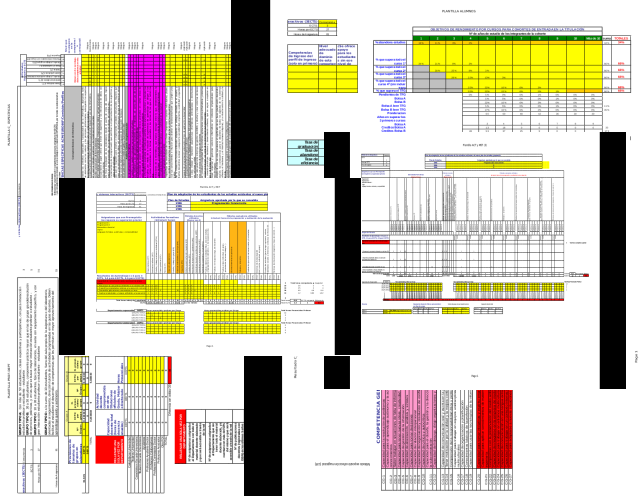
\includegraphics[width=1\textwidth]{collage.png}
	\end{center}
\end{frame}
\note{La primera aproximación al problema por parte de los docentes consistió en la elaboración de complejísimas hojas de cálculo - hasta 7 por asignatura- en las que era preciso trasladar información entre ellas mediante corta-pega. \\ Además de la frecuencia de los errores durante el alta manual de la información en las hojas, también podían ocurrir errores durante el copia-pega. Y aunque no se cometiese ningún error, comprender la información relativa a una asignatura era realmente complicado para la persona que había introducido la información, no digamos ya para una persona ajena a la misma, para quien los conceptos utilizados pueden tener significados totalmente distintos al real.}
\note{En resumen, la información contenida en las hojas de cálculo es muy proclive a padecer errores - léxicos, sintácticos y semánticos-, poco práctica - 7 hojas de cálculo para una única asignatura, una materia con 9 asignaturas ocuparía 63 hojas de cálculo, lo difícil sería no equivocarse en su interpretación- y además, la utilización de la información contenida en ellas es difícilmente aprovechable por otras aplicaciones, al carecer de sintaxis y semántica.}

%--- Unificación, formalización y ---%
%--- procesos automáticos -----------%
\begin{frame}{Motivación del trabajo}
	\begin{LARGE}
	\begin{enumerate}
		\item Formalización del conocimiento.
		\item Unificación del conocimiento.
		\item Procesos automatizados
	\end{enumerate}
	\end{LARGE}
\end{frame}
\note{Los objetivos del presente trabajo es cubrir las deficiencias observadas en el modelo de las hojas de cálculo, proporcionando un método o herramienta que facilite el paso desde el paradigma que proporcionaba el antiguo sistema de créditos hacie el nuevo ECTS. \\
Unificación del conocimiento: Resulta imprescindible que todos los actores involucrados en este cambio de paradigma tengan una visión única del universo. El conocimiento del mismo ha de ser unificado para lograr homogeneidad en los conceptos. El lograr un conocimiento único resulta básico para poder continuar trabajando en el problema. \\
Formalización del conocimiento: Es necesario formalizar ese conocimiento unificado utilizando algún lenguaje que sea lo suficientemente expresivo para el conocimiento que queremos modelar. \\}
\note{Procesos automatizados: La formalización del conocimiento nos permitirá construir o utilizar alguna herramienta que facilite el trabajo y logre minimizar la ocurrencia de fallos humanos - como el copiapega o la introducción manual de la información en las hojas de cálculo. Y si es posible, que lo haga de forma automática.}

%--- OWL, ontologías y protegé ------%
\begin{frame}{Modelización del universo}
\begin{LARGE}
	\begin{enumerate}
	\item Esquema conceptual: Ontologías.
	\pause	
	\item Lenguaje utilizado: OWL-DL.
	\pause
	\item Herramienta utilizada: Protegé.	
	\end{enumerate}
\end{LARGE}
\end{frame}
\note{Las ontologías nos permiten describir algún subconjunto del universo en función de sus propiedades y de la forma en que éstas se interrelacionan. Implica la definición de un vocabulario - Unificación del conocimiento - y reglas gramaticales - formalización del conocimiento. Este vocabulario y esta gramática otorgan a las ontologías las siguientes propiedades:\\
- Intercambio de datos entre diferentes sistemas\\
- Creación de servicios de consulta\\
- Crear bases de conocimiento reusables\\
- Ofrecer servicios de interoperabilidad entre diversos sistemas.\\
Las ontologías se expresan en lenguajes basados en conceptos lógicos, de modo que se puedan distinguir de manera inequívoca las diferentes clases, propiedades y relaciones.}
\note{Es preciso entonces utilzar un lenguaje de descripción que permita almacenar información sintáctica y semántica, para que podamos utilizar el concepto de ontología de la manera más provechosa. Existen multitudes de lenguajes semánticos. De entreo todos ellos hemos elegido OWL por ser un estándar desarrollado por W3C que permite la descripción de tipos de datos, clases, propiedades y relaciones entre ellos, propiedades de esas relaciones y clases enumeradas. Existen tres sublenguajes dentro de OWL, todos ellos desarrollados desde RDF. El más sencillo, OWL lite, no resulta lo sufientemente expresivo, y principalmente está enfocado al desarrollo de tesauros, taxonomías y otras jerarquías de clases y constantes muy simples.\\
En el lado contrario tenemos OWL-Full que por permitir la máxima expresividad y libertad sintáctica, no aporta garantías sobre su decidibilidad o completud.}
\note{Por ello hemos elegido el sulenguaje OWL-DL, que como término medio, ofrece todos los constructores de OWL pero con pequeñas condiciones, lo que le permite tener una mayor expresividad que OWL-Lite, así como las propiedades de decidibiliadd y completud a las ontologías construidas con este sub-lenguaje, lo que nos permitirá más adelante el uso de herramientas automáticas.}
\note{Protegé es un framework libre de código abierto, desarrollado conjuntamente por las universidades de Standford y Manchester (creadora de la sintaxis que lleva su nombre, válida para la construcción de ontologías en lenguaje OWL-DL.) Se ha escogido sobre otras herramientas para el desarrollo de ontologías por admitir el uso de extensiones en forma de plugins - facilitando la incorporación de herramientas que faciliten el desarrollo de la ontología-, y por su interfaz clara y fácil de utilizar, lo que le convierte en una excelente base para el desarrollo de aplicaciones o prototipos.}
%--- Clases y propiedades -----------%
\begin{frame}{Modelización del universo}
\begin{LARGE}
	Componentes de la ontología:
	\begin{itemize}
		\item Clases.
		\item Propiedades.
		\begin{itemize}
			\item Objetos
			\item Tipos de datos
		\end{itemize}
		\item Definiciones.
		\item Individuos.
	\end{itemize}		
	
\end{LARGE}
\end{frame}

\note{Las clases se pueden definir en protegé como conjuntos que contienen individuos. Las clases se describen utilizando descripciones formales que definen inequívocamente los requisitos de pertenencia a una clase. Las clases se organizan en conjuntos de superclases y subclases, que forma la taxonomía de nuestro universo en observación. Esta taxonomía puede serobtenida de manera automática por un razonador, que también puede comprobar su consistencia. Se debe tener en cuenta que todas las clases se han definido como disjuntas entre ellas de modo general, salvo las clases Competencia Especifica y Competencia General cuya disjunción se define de modo particular por ser subclases de Competencia y ser su unión disjunta.}
\note{Las propiedades son relaciones binarias entre individuos, es decir, una propiedad une dos individuos entre sí. Las propiedades pueden tener inversas, pueden ser funcionales, transitivas, simétricas. . . Estas relaciones se pueden dar tanto entre individuos de la misma clase, como entre individuos de distintas clases. Un razonador automático puede computar si una relación entre dos individuos es consistente con el resto de la ontología. Es de destacar que las propiedades únicamente se pueden establecer entre dos individuos. No existen propiedades con cardinalidad tres, lo que implicará que en el caso de que sea preciso establecer una relación a tres, sería preciso modelarlo como la relación binaria entre el producto escalar de dos de ellas sobre la tercera.}
\note{Las propiedaddes sobre tipos de datos son relaciones entre individuos y tipos de datos, de modo que se puede asociar a los individuos implicados en la relación ciertas características de tipos definidos, concretas y especificas.}
\note{Por comodidad se ha definido un tipo de datos, más por comodidad a la hora de definir las clases y propiedades, que por que sea realmente necesario a la hora del desarrollo de la ontología. En el caso de que definiésemos un tipo de datos cuya primitiva no fuese alguno de los tipos de datos definidos en el estándar de OWL2, el lenguaje de la ontología pasaría a ser OWL-Full, con lo que no podríamos realizar razonamiento alguno sobre dicha ontología, perdiendo una cualidad básica de las que buscamos con el desarrollo del
presente trabajo. El tipo de datos tipoCredito nos es útil para poder almacenar los créditos de materias y asignaturas, y si bien puede ser prescindible, me ha parecido útil restringir el rango de los datos únicamente al conjunto de los decimales positivos como una forma de evitar que el usuario de la ontología pueda completarla con datos erróneos.}
\note{Los individuos representan objetos de la ontología en el dominio que estamos estudiando. Son instancias de objetos pertenecientes a alguna de las clases definidas en la ontología. Protegé no hace uso del Unique Name Assumption, es decir, para protegé dos individuos pueden referirse al mismo objeto del mundo real, salvo que se especifique lo contrario. Esta es una consecuencia de las ontologías OWL: todo lo que no sea dicho de forma explícita puede ser cierto. El hecho de que no especifiquemos si dos individuos son o no los mismos, significa que pueden o no serlo, para ese dominio.}

%--- Definición de Asignatura en sintaxis Manchester ---%
\lstset{inputencoding=latin1}
\lstset{language=protege,basicstyle=\sffamily,columns=flexible,mathescape}
\begin{frame}{Modelización del universo}
	\begin{LARGE}
		Definición de Asignatura en sintaxis Manchester:
	\end{LARGE}
	\begin{scriptsize}
\lstinputlisting[breaklines,language=protege,literate=,linerange=Class:\ ects:Asignatura-only\ ects:Caracter]{../Texto/t-box.ms} 	
	\end{scriptsize}
\end{frame}
\note{Esta es la descripción de la clase asignatura realizada en sintaxis Manchester. Más allá del proceso automático que después podamos realizar utilizando ontologías, destaca a primer golpe de vista la claridad y sencillez de la descripción de una asignatura utilizando un lenguaje formal, contra lo complicado de comprender qué es una asignatura utilizando una herramiento no apropiada como puedan ser las hojas de cálculo presentadas al inicio de esta exposición.}


%--- Definición de una propiedad y un tipo de datos en Manchester ---%
\lstset{inputencoding=latin1}
\lstset{language=protege,basicstyle=\sffamily,columns=flexible,mathescape}
\begin{frame}{Modelización del universo}
	\begin{LARGE}
		Ejemplo de Propiedades y tipo de datos
	\end{LARGE}
	\begin{scriptsize}
		\begin{columns}[t]
			\column{0.5\textwidth}
\lstinputlisting[breaklines,language=protege,literate=,linerange=ObjectProperty:\ ects:AS\_formaParteDe\_MA-ects:MA\_constaDe\_AS]{../Texto/t-box.ms} 	
			\column{0.5\textwidth}
\lstinputlisting[breaklines,language=protege,literate=,linerange=DataProperty:\ ects:AS\_Creditos-ects:tipoCredito]{../Texto/t-box.ms}
		\end{columns}
		\begin{center}
		\lstset{language=protege,basicstyle=\sffamily,columns=flexible,mathescape=false}
		\lstinputlisting[breaklines,language=protege,literate=,firstline=16,lastline=19]{../Texto/t-box.ms}
		\end{center}
	\end{scriptsize}
\end{frame}
\note{Habla con ángelsobre si elimino o no esta diapositiva}
\note{Y este es un ejemplo de la modelización de propiedades y tipos de datos, mucho más claro, conciso y legible que las tablas incluidas en los ficheros de excel antes mencionados.}

%--- Instancia del plan de estudios -%
\lstset{inputencoding=latin1}
\lstset{language=protege,basicstyle=\sffamily,columns=flexible,mathescape}
\begin{frame}[fragile]{Aplicaciones del diseño}
	\begin{LARGE}
		Instancia de una asignatura:
	\end{LARGE}
	\begin{footnotesize}
\lstinputlisting[breaklines,language=protege,literate=,linerange=Individual:\ AS\-Concurrencia-xsd:string]{../Texto/a-box.ms} 	
	\end{footnotesize}
\end{frame}
\note{Como vemos hemos cumplido algunos de los primeros objetivos del trabajo. Hemos logrado, a través de la descripción de una ontología a través de un lenguaje formal (OWL-DL), crear un marco de conocimiento único, sin ambigüedades, y con una expresividad superior a la facilitada por las hojas de cálculo utilizadas en un principio. Ahora veremos cómo incrementar la aplicabilidad del trabajo incorporando herramientas automáticas a la ontología.}


\begin{frame}{Aplicaciones del diseño}
\begin{LARGE}
	Aplicaciones automáticas:
	
	Razonadores (FaCT++, HermiT), editores (ACE View, ChangeView, Hypergraph DB), visores (CloudViews, Matrix, NavigOWL, Ontograf, OWLGrEd, SOVA, DL-Query, Cardinality view, Tree views, OWLDoc, OWLViz, OWLPropViz, OWLDiff), transformacion (OWL2RDB).
\end{LARGE}
	
\begin{center}
	{\Huge ¡¡Wiki semántica!!}
\end{center}
\note{quédate con la idea de las dos vueltas, de cómo se ha llegado hasta la wiki (que no era el destino inicialmente), de porqué, de lo que hay y lo queda por hacer. Y porqué es útil e importante.}
\end{frame}

%\begin{frame}{Aplicaciones del diseño}
%	{\Huge ¡Wiki semántica¡}
%\end{frame}

\begin{frame}{Aplicaciones del diseño}
\begin{LARGE}
	Metas alcanzadas:
	\begin{enumerate}
		\item Coherencia con el marco legislativo.
		\item Ayuda al diseño de los itinerarios formativos.
		\item Aplicabilidad por el personal docente.
		\item Seguimiento de los planes docentes.
		\item Orientación al alumno en la elección de centro y estudios.
	\end{enumerate}
	\note{Incluye un punto de vista más personal. habla de la evolución que ha habia desde el comienzo del tfc hasta el fnal, de cómo también ha evolucionado el trabajo, de los tropiezos que hemos tenido y dificultades que tendría su implantación, y cómo se ha solucionado. Debe de ser unas conclusiones con algo de contenido personal.}
\end{LARGE}
\end{frame}

\begin{frame}{Trabajo a futuro}
\begin{LARGE}
	\begin{itemize}
		\item Mejoras en la ontología.
		\item Integración de OWL y Wiki semántica.
		\item Razonadores automáticos sobre la wiki.
	\end{itemize}
\end{LARGE}
\end{frame}

\begin{frame}[c]{}
	\begin{Huge}
	\begin{center}
		Gracias por su atención.
	\end{center}
	\end{Huge}
\end{frame}

\end{document}
